\documentclass[a4paper, 10pt]{article}

\usepackage[utf8]{inputenc}
\usepackage[italian]{babel}
\usepackage{amsmath}
\usepackage{amssymb}
\usepackage{amsthm}
\usepackage[makeroom]{cancel}
\usepackage{mathtools}
\usepackage{hyperref}
\usepackage[]{acronym}
\usepackage{syntax}
\usepackage{newfloat}
\usepackage{float}
\usepackage{listings}
%\usepackage[LGRgreek]{mathastext}
\usepackage[osf,sc]{mathpazo}
\usepackage{eulervm}
\usepackage{MnSymbol}
\usepackage{listings}
\usepackage{caption}
\usepackage{color}
\usepackage[dvipsnames]{xcolor}
\usepackage{algorithm}% http://ctan.org/pkg/algorithms
\usepackage{algpseudocode}% http://ctan.org/pkg/algorithmicx

\title{Relazione per l'approfondimento su Computational Tree Logic}
\author{Filippo Mameli, Federico Schipani}
\makeindex

\let\syntleft\relax
\let\syntright\relax
\grammarparsep=30pt
\DeclareFloatingEnvironment[
  fileext   = logr,
  listname  = {List of Grammars},
  name      = Grammatica,
  placement = H
]{Grammar}

\newtheorem{prop}{Proprietà}
\newtheorem{defn}{Definizione}
\newtheorem{theor}{Teorema}[section]
\numberwithin{equation}{theor}



\makeatletter
\newcommand{\newalgname}[1]{%
  \renewcommand{\ALG@name}{#1}%
}
\newalgname{Algoritmo}% All algorithms will be called "Algorithme"
\renewcommand{\listalgorithmname}{Lista di \ALG@name s}
\makeatother
\renewcommand{\lstlistingname}{Codice}
\renewcommand{\lstlistlistingname}{Lista di codici}


\begin{document}
\lstdefinestyle{customXML}{
    language=xml,
    tabsize=2,
    frame=lines,
    label=code:sample,
    frame=shadowbox,
    rulesepcolor=\color{gray},
    xleftmargin=10pt,
    framexleftmargin=15pt,
    keywordstyle=\color{blue}\bf,
    commentstyle=\color{OliveGreen},
    stringstyle=\color{red},
    numbers=left,
    numberstyle=\tiny,
    numbersep=5pt,
    breaklines=true,
    showstringspaces=false,
    basicstyle=\footnotesize,
    emph={food,name,price},emphstyle={\color{magenta}}}
\lstdefinestyle{customPY}{
    language=Python,
    tabsize=2,
    frame=lines,
    label=code:sample,
    frame=shadowbox,
    rulesepcolor=\color{gray},
    xleftmargin=10pt,
    framexleftmargin=15pt,
    keywordstyle=\color{blue}\bf,
    commentstyle=\color{OliveGreen},
    stringstyle=\color{red},
    numbers=left,
    numberstyle=\tiny,
    numbersep=5pt,
    breaklines=true,
    showstringspaces=false,
    basicstyle=\footnotesize,
    emph={food,name,price},emphstyle={\color{magenta}}}
\maketitle
\tableofcontents
\section{Introduzione a \ac*{CTL}}
\acf{CTL} è una logica proposta da Clarke e Emerson per far fronte ad alcuni problemi noti di \ac{LTL}. In \ac{LTL} il concetto di tempo è lineare, ciò vuol dire che in un determinato istante abbiamo un unico possibile futuro. Ciò comporta che una determinata formula $\phi$ è valida in uno stato $s$, se e solo se tutte le possibili computazioni che partono da quello stato soddisfano la formula. Più formalmente:
\begin{equation}\label{first}
    s \models \phi \iff \pi \models \phi \ \forall \  path \  \pi \ che\  inizia\  in\  s
\end{equation}
Come si può notare dalla Formula \eqref{first} non è possibile imporre facilmente condizioni di soddisfacibilità solo su alcuni di questi path. Dato uno stato $s$, si può verificare che solo alcune computazioni soddisfano una formula $\phi$  usando la dualità tra l'operatore universale ed esistenziale. Quindi verificare  $ s \models  \exists \phi $ corrisponde a verificare $s \models \neg \forall \neg \phi $. Se quest'ultima non è soddisfatta allora esisterà una computazione che soddisfa $\phi$, altrimenti non esisterà. \par
Non è possibile usare questo sotterfugio per proprietà più complicate. Per esempio la proprietà
\begin{prop}
\label{prop:first}
Per ogni computazione è sempre possibile ritornare in uno stato iniziale
\end{prop}
non è esprimibile in \ac{LTL}. Un tentativo potrebbe essere $\square\lozenge start$, dove $start$ indica uno stato iniziale. Tuttavia una formula di questo tipo è troppo forte, in quanto impone che una computazione ritorni sempre in uno stato iniziale, e non soltanto eventualmente. \par
\ac{CTL} risolve questi problemi introducendo una nozione di tempo che si basa sulle diramazioni. Quindi non abbiamo più un'infinita sequenza di stati, ma un infinito albero di stati. Questo comporta che in un determinato istante avremo diversi possibili futuri.\par
La semantica di questa logica è definita in termini di infiniti alberi, dove ogni diramazione rappresenta un singolo percorso. L'albero quindi è una fedele rappresentazione di tutti i possibili path, e si può facilmente ottenere srotolando il \ac{TS}.\par
In \ac{CTL} sono presenti quantificatori, definiti sui path, di tipo esistenziale ($\exists$) ed universale ($\forall$). La Proprietà $\exists\lozenge \psi$ dice che esiste una computazione che soddisfa $\lozenge\psi$, più intuitivamente vuol dire che esisterà almeno una possibile computazione nel quale uno stato $s$ che soddisfa $\psi$ verrà eventualmente raggiunto. Tuttavia questo non esclude la possibilità che ci possono essere computazioni per le quali questa proprietà non viene soddisfatta.
La proprietà \ref{prop:first} citata in precedenza è possibile ottenerla annidando quantificatori esistenziali ed universali in questo modo:
\begin{equation}
\label{second}
\forall\square\exists\lozenge start
\end{equation}
La Formula \eqref{second} si legge come: in ogni stato ($\square$) di ogni possibile computazione ($\forall$), è possibile ($\exists$) eventualmente ritornare in uno stato iniziale ($\lozenge start$).


\subsection{Sintassi di \ac{CTL}}
\ac{CTL} ha una sintassi a due livelli, dove le formule sono classificate in \textit{formule sugli stati} e \textit{formule sui path}.

\begin{Grammar}
	\begin{grammar}

	\centering
	<$\boldsymbol{\phi}$> ::= true | a | $\boldsymbol{\phi}_{1} \wedge \boldsymbol{\phi}_{2}$ | $\neg \boldsymbol{\phi}$ | $	\exists \varphi$ | $\forall \varphi$

	\end{grammar}
	\caption{Grammatica per le formule sugli stati}\label{gra:stateformulae}
\end{Grammar}
Le prime sono definite dalla Grammatica \ref{gra:stateformulae} dove $a \in AP$ e $\varphi$ è una formula sui path.
\begin{Grammar}
	\begin{grammar}

	\centering
	<$\varphi$> ::= $\bigcircle \boldsymbol{\phi}$ | $\boldsymbol{\phi}_{1}\ \boldsymbol{U}\  \boldsymbol{\phi}_{2}$

	\end{grammar}
	\caption{Grammatica per le formule sui path}\label{gra:pathformulae}
\end{Grammar}
Le \textit{formule sui path} sono invece definite dalla Grammatica \ref{gra:pathformulae}.
Intuitivamente si può dire che le formule sugli stati esprimono una proprietà su uno stato, mentre le formule sui path esprimono proprietà sui infinite sequenze di stati. Per esempio la formula $\bigcircle \phi$ è vera per un path se lo stato successivo, in quel path, soddisfa $\phi$. Una formula sugli stati può essere trasformata in una formula sui path aggiungendo all'inizio un quantificatore esistenziale ($\exists$) o universale ($\forall$). Per esempio la formula $\exists \varphi$ è valida in uno stato se esiste almeno un percorso che soddisfa $\varphi$.

\subsection{Semantica di \ac{CTL}}

Le formule \ac{CTL} sono interpretate sia sugli stati che sui path di un \ac{TS}. Formalmente, dato un \ac{TS}, la semantica di una formula è definita da due relazioni di soddisfazione: una per le formule di stato ed una per le formule di path.
Per le formule di stato è un tipo di relazione tra gli stati del \ac{TS} e la formula di stato. Si scrive che $s \models \boldsymbol{\phi}$ se e solo se la formula di stato $\boldsymbol{\phi}$ è vera nello stato $s$.\par
Per le formule di path la relazione $\models$ è una relazione definita tra un frammento di path massimale nel \ac{TS} e una formula di path. Si scrive che $\pi \models \varphi$ se e solo se il path $\pi$ soddisfa la formula $\varphi$.
\begin{defn}
Sia $a \in AP$ una proposizione atomica, $TS = (S, act, \rightarrow, I, AP, L)$ un \acf{TS} senza stati terminali, stati $s \in S$, $\boldsymbol{\phi}$, $\boldsymbol{\Psi}$ formule \ac{CTL} di stato e $\varphi$ una formula \ac{CTL} di path. La relazione di soddisfazione $\models$ per le formule di stato è definita come:
$$s \models a \iff a \in L(s)$$
$$s \models \neg \boldsymbol{\phi} \iff not\ s \models \boldsymbol{\phi}$$
$$s \models \boldsymbol{\phi} \wedge \boldsymbol{\Psi} \iff (s \models \boldsymbol{\phi})\ e\ (s \models \boldsymbol{\Psi}) $$
$$s \models \exists \varphi \iff \pi \models \varphi\ per\ alcuni\ \pi \in Paths(s)$$
$$s \models \forall \varphi \iff \pi \models\ per\ tutti\ i\ \pi \in Paths(s)$$
Per un path $\pi$, la relazione di soddisfazione $\models$ per le formule di path è definita da:
$$\pi \models \bigcircle \boldsymbol{\phi} \iff \pi[1] \models \boldsymbol{\phi}$$
$$\pi \models \boldsymbol{\phi}\ \boldsymbol{U}\  \boldsymbol{\Psi} \iff \exists j \geqslant 0.(\pi[j] \models \boldsymbol{\Psi} \wedge (\forall 0 \leqslant k < j. \pi[k] \models \boldsymbol{\phi})$$
\end{defn}
\section{Model Checking di \ac{CTL}}
Data una formula \ac{CTL} $\phi$ ed un \ac{TS} l'obiettivo dell'algoritmo di Model Checking è quello di dire se il \ac{TS} soddisfa o meno la formula. Gli algoritmi proposti lavorano su formule in \ac{ENF}, definite dalla Grammatica~\ref{gra:enf}
\begin{Grammar}
	\begin{grammar}

	\centering
	<$\phi$> ::= true | $a$ | $\phi_{1} \wedge \phi_{2}$ | $\neg \phi$ | $\exists\bigcircle\phi$ | $\exists\square\phi$ | $\exists(\phi_{1} \boldsymbol{U} \phi_{2})$

	\end{grammar}
	\caption{Grammatica delle formule in ENF}\label{gra:enf}
\end{Grammar}

il che non è limitate in quanto il Teorema~\ref{theorem:enf} dimostra che per ogni formula \ac{CTL} esiste la corrispondente formula in \ac{ENF}.
\begin{theor}
\label{theorem:enf}
Per ogni formula \ac{CTL} esiste un equivalente formula \ac{CTL} in \ac{ENF}
\end{theor}
\begin{proof}
Grazie alle leggi di dualità si ottengono delle regole di traduzione:
$$\forall\bigcircle \phi \equiv \neg \exists \bigcircle \neg \phi$$
$$\forall(\phi \boldsymbol{U} \Psi) \equiv \neg \exists( \Psi \boldsymbol{U} (\neg \phi \wedge \Psi)  )\wedge \neg\exists\square\neg\Psi$$
\end{proof}
\begin{algorithm}
\caption{Algoritmo di model checking base per \ac{CTL}}
\label{alg:base}
\begin{algorithmic}[1]
\Procedure{CTLModelChecking}{$TS, \phi$}
\ForAll{$i \leq |\phi|$}
\ForAll{$\Psi \in Sub(\phi)\ con\ |\Psi| = i$}
\State calcola $Sat(\Psi)$ da $Sat(\Psi^{'})$
\EndFor
\EndFor
\State \textbf{return} $I  \subseteq Sat(\phi)$
\EndProcedure
\end{algorithmic}
\end{algorithm}
%correggere riferimento non funzionante
L'algoritmo base, mostrato in Algoritmo \ref{alg:base}, risolve ricorsivamente il problema di verificare se un determinato \ac{TS} soddisfa una formula $\phi$.
Fondamentalmente il calcolo consiste in un attraversamento dalle foglie alla radice dell'albero di parsing della formula sugli stati $\phi$. In questo albero i nodi rappresentano le sottoformule $\Psi$ di $\phi$, mentre le foglie rappresentano le proposizioni atomiche $a \in AP$ e la costante $true$.
Durante la computazione vengono calcolati ricorsivamente gli insiemi $Sat{\Psi}$ per ogni sottoformula $\Psi$ di $\phi$. Ad ogni passo, per stabilire quali sono gli stati che soddisfano un nodo $v$, si combinano le valutazioni (già effettuate) dei suoi nodi figli. Il tipo di computazione quando si raggiunge il nodo $v$ dipende dal tipo di operatore che contiene, che può essere $\wedge$, $\exists\bigcircle$ oppure $\exists\boldsymbol{U}$.\par
Il seguente teorema definisce come vengono generati gli insiemi di sottoformule.


\begin{theor}
\label{eq:teoremaCaratterizzazione}
Sia $TS = (S, Act, \rightarrow, I, AP, L)$ un \ac{TS} senza stati terminali. Per tutte le formule \ac{CTL} $\phi$, $\Psi$ su AP è vero che:

\begin{equation}\label{eq:te1}
Sat(true) = S
\end{equation}

\begin{equation}\label{eq:te2}
Sat(a) = \{s \in S | a \in L(s)\}
\end{equation}

\begin{equation}\label{eq:te3}
Sat( \phi \wedge \Psi) = Sat(\phi)  \cap Sat(\Psi)
\end{equation}

\begin{equation}\label{eq:te4}
Sat(\neg \phi) = S \backslash Sat(\phi)
\end{equation}

\begin{equation}\label{eq:te5}
Sat(\exists\bigcircle\phi) = \{s \in S | Post(s) \cap Sat(\phi) \neq \emptyset\}
\end{equation}

\begin{equation}\label{eq:te6}
\begin{aligned}
Sat(\exists(\phi \boldsymbol{U} \Psi))\ \text{è il più piccolo sottoinsieme T di S tale per cui } \\
(Sat(\Psi) \subseteq T \wedge (s \in Sat(\phi) \wedge Post(s) \cap T \neq \emptyset)) \implies s \in T
\end{aligned}
\end{equation}

\begin{equation}\label{eq:te7}
\begin{aligned}
Sat(\exists(\square\phi)) \text{è il più grande sottoinsieme T di S tale che} \\
T \subseteq Sat (\phi) \wedge s \in T \implies Post(s) \cap T \neq \emptyset
\end{aligned}
\end{equation}
\end{theor}



Le caratterizzazioni fornite dal Teorema \ref{eq:teoremaCaratterizzazione} forniscono una base per la costruzione di algoritmi per calcolare gli insiemi di soddisfacibilità per i vari operatori. \par
Per l'operatore Until $\boldsymbol{U}$ la \eqref{eq:te6} del Teorema \ref{eq:teoremaCaratterizzazione} suggerisce di usare una procedura iterativa tale per cui $T_{0} = Sat(\Psi)$ e $T_{i+1} = T_{i} \cup \{s \in Sat{\phi} | Post(s) \cap T_{i} \neq \emptyset \}$. L'insieme $T_{i}$ contiene tutti gli stati che possono raggiungere uno stato $s \in Sat{\Psi}$ in $i$ passi attraverso path che passano per stati $s^{1} \in Sat{\psi}$.

\begin{algorithm}
\caption{Algoritmo per $Sat(\exists(\phi \boldsymbol{U} \Psi)$)}
\label{alg:until}
\begin{algorithmic}[1]
\Procedure{ComputeExistsUntil}{$TS, \phi \boldsymbol{U} \Psi$}
\State E $:= Sat(\Psi)$
\State T $:=$E
\While{$E \neq \varnothing $}
\State let $s^{1} \in E$
\State $E:=E \backslash \{s^{1}\}$
\ForAll{ $s \in Pre(s^{1})$}
\If{$s \in Sat(\phi)\backslash T$}
\State $E:= E \cup \{s\}$
\State $T:=T \cup\{s\}$
\EndIf
\EndFor
\EndWhile
\State \textbf{return} $T$
\EndProcedure
\end{algorithmic}
\end{algorithm}
L'Algoritmo \ref{alg:until} parte calcolando tutti gli stati che soddisfano $\Psi$, che vengono poi copiati in due insiemi: $E$ e $T$. Successivamente parte un ciclo che effettua una ricerca andando ad analizzare i predecessori degli stati. In questo ciclo viene preso un elemento $s'$ dall'insieme $E$ e ne vengono analizzati i predecessori. Se uno stato $s$ appartiene a  $Pre(s') \backslash T$ allora viene inserito in $E$ ed in $T$. Alla fine l'insieme T conterrà tutti gli stati che soddisfano la formula  $\exists(\phi \boldsymbol{U} \Psi)$.\par
L'algoritmo per calcolare $Sat(\exists \square \phi)$ sfrutta la caratterizzazione fornita da \ref{eq:te7}. L'idea base è computare $Sat(\exists \square \phi)$ iterativamente in questo modo:
$$T_{0} = Sat(\phi)\ e \ T_{i+1} = T_{i} \cap \{s \in Sat(\phi)\  |\ Post(s) \cap T_{i} \neq \emptyset\}$$
\begin{algorithm}
\caption{Algoritmo per $Sat(\exists \square \phi)$}
\label{alg:always}
\begin{algorithmic}[1]
\Procedure{ComputeExistsAlways}{$TS, (\exists \square \phi)$}
\State E $:= S \backslash Sat(\phi)$
\State T $:=Sat(\phi)$
\ForAll{$s \in Sat(\phi)$}
\State $count[s] := |Post(s)|$
\EndFor
\While{$E \neq \varnothing $}
\State let $s^{1} \in E$
\State $E:=E \backslash \{s^{1}\}$
\ForAll{ $s \in Pre(s^{1})$}
\If{$s \in T$}
\State $count[s] := count[s]-1$
\If{$count[s] = 0$}
\State $T := T \backslash \{s\}$
\State $E := E \cup \{s\}$
\EndIf
\EndIf
\EndFor
\EndWhile
\State \textbf{return} $T$
\EndProcedure
\end{algorithmic}
\end{algorithm}
L'algoritmo \ref{alg:always} realizza questa procedura con una ricerca volta all'indietro che inizia con
$$T = Sat(\phi) \qquad e \qquad E = S\backslash Sat(\phi)$$
in questo caso $T$ è uguale a $T_{0}$ ed $E$ contiene tutti gli stati per cui $\exists \square \phi$ è falsa. Durante la ricerca gli stati $s \in T$ che non soddisfano $\exists \square \phi$ vengono rimossi se $Post(s) \cap T = \emptyset$.
Questa verifica è resa possibile da un array chiamato
$count[s]$ definito $\forall s \in Sat(\phi)$ che conta quanti successori ha lo stato $s$. Questo contatore verrà decrementato ogni volta che uno stato contenuto nei predecessori di uno stato $s' \in E$ è anche in $T$. Quando il contatore è $0$ lo stato verrà marcato come stato che non soddisfa $\forall s \in Sat(\phi)$, quindi sarà rimosso da $T$ ed aggiunto ad $E$.



%\begin{algorithm}
%\label{alg:alternativealways}
%\caption{Algoritmo alternativo per $Sat(\exists \square \phi)$}
%\begin{algorithmic}[1]
%\Procedure{AlternativeComputeExistsAlways}{$TS, (\exists \square \phi)$}
%\State $S^{1} := Sat{\phi}$
%\State $\rightarrow^{1} := \rightarrow \cap(S^{1} \times Act \times S^{1})%$
%\State $I^{1} := I \cap S^{1}$
%\State $L^{1}(s) := L(s) | s \in S^{1}$
%\State $TS[\phi] := (S^{1}, Act, \rightarrow^{1}, I^{1}, AP, L^{1}) $
%\State $T := ComputeSSC(TS[\phi])$
%\State return $Reach(I, T)$
%\EndProcedure
%\end{algorithmic}
%\end{algorithm}



\subsection{Complessità dell'algoritmo}
\begin{theor}
Per un \acf{TS} con N stati e K transizioni, ed una formula CTL $\phi$, il problema di $TS \models \phi$ può essere risolto in tempo $$O((N+K) \cdot |\phi|)$$
\end{theor}
\begin{proof}
La complessità in tempo di questo algoritmo è determinata come segue. Sia \ac{TS} un \acf{TS} finito con N stati e K transizioni. Sotto l'assunzione che l'insieme di predecessori di uno stato sono rappresentati da una \textit{Linked List}, la complessità degli Algoritmi \ref{alg:always} e \ref{alg:until} sono $O(N+K)$. Visto che la computazione del $Sat(\phi)$ viene effettuata in una maniera \textit{bottom-up} la complssità risulta lineare nella dimensione della formula, quindi la complessità dell'algoritmo \ref{alg:base} è data da $$O((N+K) \cdot |\phi|) $$
\end{proof}
Va però ricordato che l'algoritmo proposto lavora con formule in \ac{ENF}, il che può portare ad una crescita esponenziale della dimensione della formula. Fortunatamente però esistono algoritmi per calcolare gli insiemi di stati soddisfatti per formule non in ENF, che hanno complessità $O(N+K)$.

\section{Model Checker in Python per \ac{CTL}}
Il programma è stato realizzato utilizzando Python con l'ausilio delle librerie \texttt{pyparser} e \texttt{networkx}. La prima libreria è stata usata per definire la grammatica di \ac{CTL} ed effettuare il parsing di una formula passata in input come una stringa.
La seconda libreria è stata invece utilizzata per la rappresentazione dei \ac{TS}. Questa libreria contiene molte funzioni che si sono rivelate essenziali durante lo sviluppo del model checker, come per esempio la possibilità di ottenere liste di predecessori e successori di uno stato con una sola riga di codice.
\subsection{Come vengono rappresentati i \ac{TS}}
Un \acf{TS} viene rappresentato come un grafo $G$ dove i nodi sono gli stati del \ac{TS} e gli archi sono rappresentati dagli archi del \ac{TS}. Più formalmente:
\begin{defn}
Dato un \acf{TS} = $\{S, Act, \rightarrow, I, AP, L\}$ si considera il grafo sottostante $G = (V,E)$ tale che $V = S$ e $E = \{ (s, s')\ \in S x S|\ s' \in Post(s)\}$
\end{defn}
Grazie alla libreria \href{https://networkx.github.io}{\texttt{networkx}} è possibile leggere un grafo da un file \ac{XML} in linguaggio \href{https://gephi.org/gexf/format/}{\ac{GEXF}}.
\ac{GEXF} è un linguaggio usato per la definizione di strutture complesse, come grafi, in maniera semplice. Un esempio di grafo in \ac{GEXF} è mostrato in Codice~\ref{code:esgrafo}. Questo grafo è di tipo diretto ed è formato da due nodi e un arco che li collega, il primo nodo ha label \texttt{Hello} ed il secondo ha label \texttt{World}.

\lstinputlisting[style=customXML, caption = Esempio di grafo rappresentato in XML, label = {code:esgrafo}]{CodiceRelazione/esempiografo.xml}

Per leggere il grafo in Python sono sufficienti poche righe di codice, mostrate in Codice~\ref{code:letturagrafo}.
\lstinputlisting[style=customPY, caption = Lettura di un file \ac{GEXF}, label = {code:letturagrafo}]{CodiceRelazione/letturagrafo.py}
\par
Un \ac{TS} è rappresentato da un nodo principale \texttt{graph} con attributi \texttt{mode} impostato a \texttt{static} e \texttt{defaultedgetype} impostato a \texttt{directed}. A sua volta questo nodo conterrà due nodi figli chiamati \texttt{nodes} e \texttt{edges}, che conterranno a loro volta una lista di nodi e di archi.
Uno stato di un \ac{TS} viene rappresentato assegnando, nel file \ac{GEXF} un figlio \texttt{node} al padre \texttt{nodes}, con attributo \texttt{id} scelto arbitrariamente e attributo \texttt{label} contenente le proposizioni atomiche che sono soddisfatte dallo stato considerato. Per rappresentare uno stato iniziale del \ac{TS} è sufficiente anteporre al \texttt{id} dello stato una \texttt{S}.
Un arco è semplicemente rappresentato da un figlio \texttt{edge} del nodo padre \texttt{edges}. Gli attributi di un nodo \texttt{edges} sono \texttt{id}, \texttt{target} e \texttt{source}. L'identificativo può essere scelto aribitrariamente, mentre \texttt{target} e \texttt{source} sono rispettivamnete la destinazione e la sorgente dell'arco.

\subsection{Come vengono rappresentate le formule}
Sono state definite due grammatiche, una per le formule \ac{CTL} una per quelle in \ac{ENF} riportata in Grammatica~\ref{gra:enfs}.
Una formula del tipo $\exists \square \forall(a U b) $ può essere scritta utilizzando la grammatica riportata in Grammatica~\ref{gra:ctls} in questo modo:
$$ [] (a \ FU \ b) $$

Si distinguono gli operatori unari, come la negazione, e gli operatori binari, come \& o UNTIL.
Più specificatamente si indica gli operatori unari:
\begin{itemize}
  \item $ \neg \varphi $ con !$\varphi $
  \item $ \exists \square \varphi$ con [] $\varphi $
  \item $ \exists \bigcircle \varphi$ con NEXT $\varphi $
  \item $ \exists \lozenge \varphi$ con EE $\varphi $
  \item $ \forall \lozenge \varphi$ con FE $\varphi $
  \item $ \forall \square \varphi$ con FA $\varphi $
  \item $ \forall \bigcircle \varphi$ con FN $\varphi $
\end{itemize}
Per gli operatori binari:
\begin{itemize}
  \item $ \exists (\boldsymbol{\varphi}_{1} \ \boldsymbol{U} \ \boldsymbol{\varphi}_{2})$ con $ \boldsymbol{\varphi}_{1} \ UNTIL \ \boldsymbol{\varphi}_{2}$
  \item $ \boldsymbol{\varphi}_{1} \ \& \ \boldsymbol{\varphi}_{2}$ con $ \boldsymbol{\varphi}_{1} \ \& \ \boldsymbol{\varphi}_{2}$
  \item $ \forall (\boldsymbol{\varphi}_{1} \ \boldsymbol{U} \ \boldsymbol{\varphi}_{2})$ con $ \boldsymbol{\varphi}_{1} \ FU \ \boldsymbol{\varphi}_{2}$
\end{itemize}
Le variabili atomiche si possono scrivere utilizzando concatenazioni di lettere minuscole dell'alfabeto o numeri interi.
Si può scrivere ad esempio $(a \ \& \ b)$, ma anche $(a1 \ \& \ b32) $ oppure $ (zty \ \& \ x6)$.

In molti casi si possono omettere le parentesi, ad esempio si può scrivere $ a \ UNTIL \ b \ UNTIL \ c$ che sarà valutata come $ (a \ UNTIL \ b) \ UNTIL \ c$.

Sono invece scartate formule con due o più operatori unari consecutivi in cui non si specifica le parentesi, ad esempio $[] !a$ non sarà valutata mentre la formula $ [] (!a)$ sì.
\begin{Grammar}
	\begin{grammar}
	\centering

  <$atom$> ::= true | a \\
  <$\boldsymbol{\varphi}$> ::= atom | $\neg \varphi$ | $[] \varphi$ | NEXT $\varphi$ | EE $\varphi$ | FE $\varphi$ | FA $\varphi$ | FN $\varphi$ | $\boldsymbol{\phi}$\\
	<$\boldsymbol{\phi}$> ::= $\boldsymbol{\varphi}_{1} \ \& \ \boldsymbol{\varphi}_{2}$ | $\boldsymbol{\varphi}_{1} \ UNTIL \ \boldsymbol{\varphi}_{2}$ | $\boldsymbol{\varphi}_{1} \ FU \ \boldsymbol{\varphi}_{2}$ \\

  \end{grammar}
	\caption{Grammatica per le formule \ac{CTL}}\label{gra:ctls}
\end{Grammar}
\begin{Grammar}
	\begin{grammar}
	\centering
  <$atom$> ::= true | a \\
  <$\boldsymbol{\varphi}$> ::= atom | $\neg \varphi$ | $[] \varphi$ | NEXT $\varphi$ | $\boldsymbol{\phi}$\\
	<$\boldsymbol{\phi}$> ::= $\boldsymbol{\varphi}_{1} \ \& \ \boldsymbol{\varphi}_{2}$ | $\boldsymbol{\varphi}_{1} \ UNTIL \ \boldsymbol{\varphi}_{2}$\\
	\end{grammar}
	\caption{Grammatica per le formule \ac{ENF}}\label{gra:enfs}
\end{Grammar}
\subsubsection{Il parsing della formula}
\label{subsub:parsingformula}
Per analizzare la formula si utilizza la libreria \texttt{pyparsing}. Si possono definire facilmente delle grammatiche e ricavare
da una formula in notazione infissa uno stack in notazione postfissa, contenente tutti gli elementi della formula.

Nel Codice~\ref{code:ctlParser} dalla linea 31 alla 42 si definiscono gli operatori unari e le variabili atomiche.
Gli operatori unari possono essere:
\begin{itemize}
  \item un operatore e la variabile atomica semplice, es. !a
  \item un operatore e la variabile atomica con le parentesi, es. !(a)
  \item un operatore e un'espressione tra parentesi, es. !(a \& b)
\end{itemize}
Le variabili atomiche sono "TRUE" oppure tutte le possibili concatenazioni di lettere minuscole o numeri interi quindi: $ ((a..z)^*(1..9)^*)^*$.

Alla linea 48 nella variabile \texttt{factor} si salvano le possibili operazioni binarie utilizzando la funzione di \texttt{pyparsing} \texttt{ZeroOrMore}.
Infatti nella formula possono esserci zero operazioni di \& o UNTIL e quindi factor sarà formato solo da \texttt{atoms} cioè le combinazioni di espressioni con operazioni unarie o variabili atomiche.
Se presenti, le operazioni binarie sono del tipo:
\begin{itemize}
  \item un operatore e le due espressioni, es. a \& !b
  \item una serie di operatori e le espressioni, es. a \& b \& (c UNTIL d) \& e
\end{itemize}
Ad ogni elemento è associata un'azione che inserisce il valore nello stack, es \& ha \texttt{pushBinary}.
La funzione \texttt{parseString} (linea 54) identifica gli elementi appartenenti alla formula e invoca le azioni al momento dell'idividuazione dell'espressione.
\lstinputlisting[firstnumber= 31,firstline = 31, lastline = 55, style = customPY, caption = Parser CTL, label = {code:ctlParser}]{CodiceRelazione/CTLParser.py}
\subsubsection{La conversione in ENF}
Per convertire la formula in \ac{ENF} si crea con stessa metodologia usata nel parsing uno stack contenente gli elementi della formula in notazione postfissa,
e in aggiunta si valuta lo stack per restituire la stringa convertita.
Una volta creato lo stack si invoca la funzione \texttt{evaluateStack} che ricorsivamente costruisce la stringa di output.
In Codice~\ref{code:enfConverter} si mostrano i casi base in cui non si fanno modifiche alla formula.
\lstinputlisting[firstnumber= 77,firstline = 77, lastline = 84, style = customPY, caption = ENF Converter, label = {code:enfConverter}]{CodiceRelazione/ENFConverter.py}
In Codice~\ref{code:enfConverterFU} si mostra invece la conversione nel caso di FU(Forall until), dove viene utilizzata la seguente equivalenza:
$$\forall(\phi \boldsymbol{U} \Psi) \equiv \neg \exists( \Psi \boldsymbol{U} (\neg \phi \wedge \Psi)  )\wedge \neg\exists\square\neg\Psi$$
per convertire la seguente formula:

\centerline{$\phi$ FU $\Psi$}
nella controparte in \ac{ENF}:
\centerline{!( $\Psi$ UNTIL (!$\phi$ \& $\Psi$)) \& !([]!($\Psi$))}

\lstinputlisting[firstnumber= 102,firstline = 102, lastline = 106, style = customPY, caption = ENF Converter, label = {code:enfConverterFU}]{CodiceRelazione/ENFConverter.py}

\subsection{Gli algoritmi di model checking}
Il model checker vero e proprio è definito come una classe in python, che per essere istanziata necessita di un \ac{TS} e di una formula \ac{CTL} in ENF. Quindi in fase di costruzione si occuperà di leggere il file \ac{GEXF} e convertire la formula in notazione postfissa, memorizzandola in uno stack, come descritto in Sottosezione \ref{subsub:parsingformula}.\par
Una volta creata l'istanza della classe \texttt{CTLModelChecker} è necessario chiamare la funzione mostrata in Codice~\ref{code:basefunction}, che rappresenta una possibile implementazione dell'Algoritmo \ref{alg:base}.
\lstinputlisting[firstline = 22, lastline = 47, style=customPY, caption = Funzione che effettua il model checking base, label = {code:basefunction}]{CodiceRelazione/modelchecker.py}
Questa funzione scorre iterativamente la formula effettuando diverse operazioni in base all'elemento analizzato, effettuandone così la valutazione.
Il caso base è quando viene analizzato un singoletto, ovvero una singola proposizione senza operatori logici. In questo caso viene richiamato il metodo \texttt{__checkSingle()}, mostrato in Codice~\ref{code:checksingle}, il quale ritornerà un insieme di stati che soddisfano il singoletto. Questo insieme sarà aggiunto ad una pila temporanea, che alla fine conterrà come singolo elemento solamente l'insieme di stati che soddisfano la formula data in input.
\lstinputlisting[firstline = 97, lastline = 102, style = customPY, caption = Funzione per il calcolo dell'insieme di soddisfacibilità di una singola proposizione, label = {code:checksingle}]{CodiceRelazione/modelchecker.py}
Il compito di questo metodo è molto semplice, itera la lista dei nodi e verifica se la proposizione atomica in questione è presente all'interno dell'attributo \texttt{label} del nodo preso in considerazione.\par
Se durante la valutazione della formula si incorre in un operatore bisogna estrarre dalla pila uno, o due insiemi di stati soddisfatti ed effettuare l'operazione. L'operatore più semplice da gestire è il NOT, in quanto, come mostrato in Codice~\ref{code:not} è sufficiente sottrarre a tutti gli stati del \ac{TS} gli stati passati in input alla funzione \texttt{__checkNot()}.
\lstinputlisting[firstline = 107, lastline = 110, style = customPY, caption = Funzione per il calcolo del NOT, label = {code:not}]{CodiceRelazione/modelchecker.py}
Il calcolo dell'AND richiede due insiemi di stati, che saranno estratti dalla pila e passati in input alla funzione mostrata in Codice~\ref{code:and}. Questa funzione trasforma in oggetti di tipo \texttt{set} le due liste passate in input, ne effettua l'intersezione e le ritorna sottoforma di lista.
\lstinputlisting[firstline = 104, lastline = 105, style = customPY, caption = Funzione per il calcolo del AND, label = {code:and}]{CodiceRelazione/modelchecker.py}
L'operatore $\bigcircle$ richiede solamente una lista di stati e iterando sulla lista dei nodi effettua l'operazione di intersezione tra i successori del nodo preso in considerazione e la lista di stati passata in input. Se la dimensione dell'insieme risultante è maggiore di 0 allora il nodo verrà aggiunto alla lista di stati che soddisfa la formula per cui è stato chiamato il metodo. L'implementazione di questa funzione è mostrata in Codice~\ref{code:next}.
\lstinputlisting[firstline = 75, lastline = 81, style = customPY, caption = Funzione per il calcolo del NEXT, label = {code:next}]{CodiceRelazione/modelchecker.py}

Nel caso in cui si incorre nell'operatore $\square$ viene richiamato il metodo \texttt{__checkAlways()}, che prende in input una singola lista di stati. Questo metodo è una implementazione dell'Algoritmo \ref{alg:always} ed è mostrato in Codice~\ref{code:always}
\lstinputlisting[firstline = 58, lastline = 73, style = customPY, caption = Funzione per il calcolo del ALWAYS, label = {code:always}]{CodiceRelazione/modelchecker.py}
Per l'operatore $\boldsymbol{U}$ è stato implementato l'Algoritmo \ref{alg:until}, mostrato in Codice~\ref{code:until}.
\lstinputlisting[firstline = 82, lastline = 92, style = customPY, caption = Funzione per il calcolo del UNTIL, label = {code:until}]{CodiceRelazione/modelchecker.py}
L'ultima operazione effettuata dall'Algoritmo \ref{alg:base} è verificare se gli stati iniziali sono un sottoinsieme degli stati soddisfatti dalla formula. Il Codice \ref{code:basefunction} effettua questa operazione alla riga 26.
\subsection{Una versione migliorata del Model Checker}
Con lo scopo di migliorare le prestazioni dell'algoritmo di Model Checking è stata sviluppata un'ulteriore versione che fa uso di una tecnica di caching. Usando questa tecnica ad ogni passo viene memorizzato in un dizionario il risultato delle sottoformule valutate. In questo modo, se la formula contiene più sottoformule uguali non è necessario rivalutarle ogni volta, ma basta accedere al dizionario per prenderne il risultato.
Per realizzare questa ottimizzazione è stato inserito un dizionario all'interno della classe, ed il metodo \texttt{iterativeCheckFormula} mostrato in Codice \ref{code:basefunction} è stato modificato. Il nuovo metodo \texttt{iterativeCheckFormula} per ogni elemento dello stack verifica prima se è già stato valutato effettuando un accesso nel dizionario. Nel caso in cui sia già stato valutato non effettua una chiamata al metodo che si occupa della valutazione, ma aggiunge alla pila degli stati soddisfatti l'elemento corrispondente del dizionario. L'implementazione di questa funzione è mostrata in Codice~\ref{code:basecache}.
\lstinputlisting[firstline = 24, lastline = 66, style = customPY, caption = Funzione per il model checking base ottimizzata con la tecnica del caching, label = {code:basecache}]{CodiceRelazione/modelcheckercaching.py}

\section{Esempi di utilizzo del Model Checker di \ac{CTL} in Python}
Per provare il model checker sono state verificate le formule di esempio analizzate nel libro di testo, inoltre è stato sviluppato un piccolo script Python
che costruisce il \ac{TS} che modella il problema dei filosofi a cena.
\subsection{Formula $ \exists \lozenge  \phi$}
Sul \ac{TS} riportato in Figura~\ref{ts6} è stato verificata la formula $ \exists \lozenge  \phi$ in cui
$$ \phi = ((a\ =\ c)\ or\ (a\ !=\ b))$$
cioè  $\phi = !(!(a \ \& \ c \ \& \ !b) \ \& \ !(!a \ \& \ !c \ \& \ b))$.
La formula nella sintassi descritta in Grammatica~\ref{gra:ctls} equivale a

$$ \text{EE} (!(!( a\ \&\ c\ \&\ !b)\ \&\ !( !a\ \&\ !c\ \&\ b)))$$
 e sarà tradotta in \ac{ENF} in \\
$$\text{TRUE UNTIL} (!(!(a\ \&\ c\ \&\ !(b))\ \&\ !(!(a)\ \&\ !(c)\ \&\ b)))$$
 per poi essere passata al modelChecker. Questo restituisce il risultato della valutazione e l'insieme di stati soddisfatti cioè:

$$(\text{False}, ['5', '4', '6', '7'])$$
Si può anche utilizzare l'insieme ricavato per mostrare visivamente gli stati soddisfatti come mostrato in Figura~\ref{tsResult1}.
\begin{figure}
  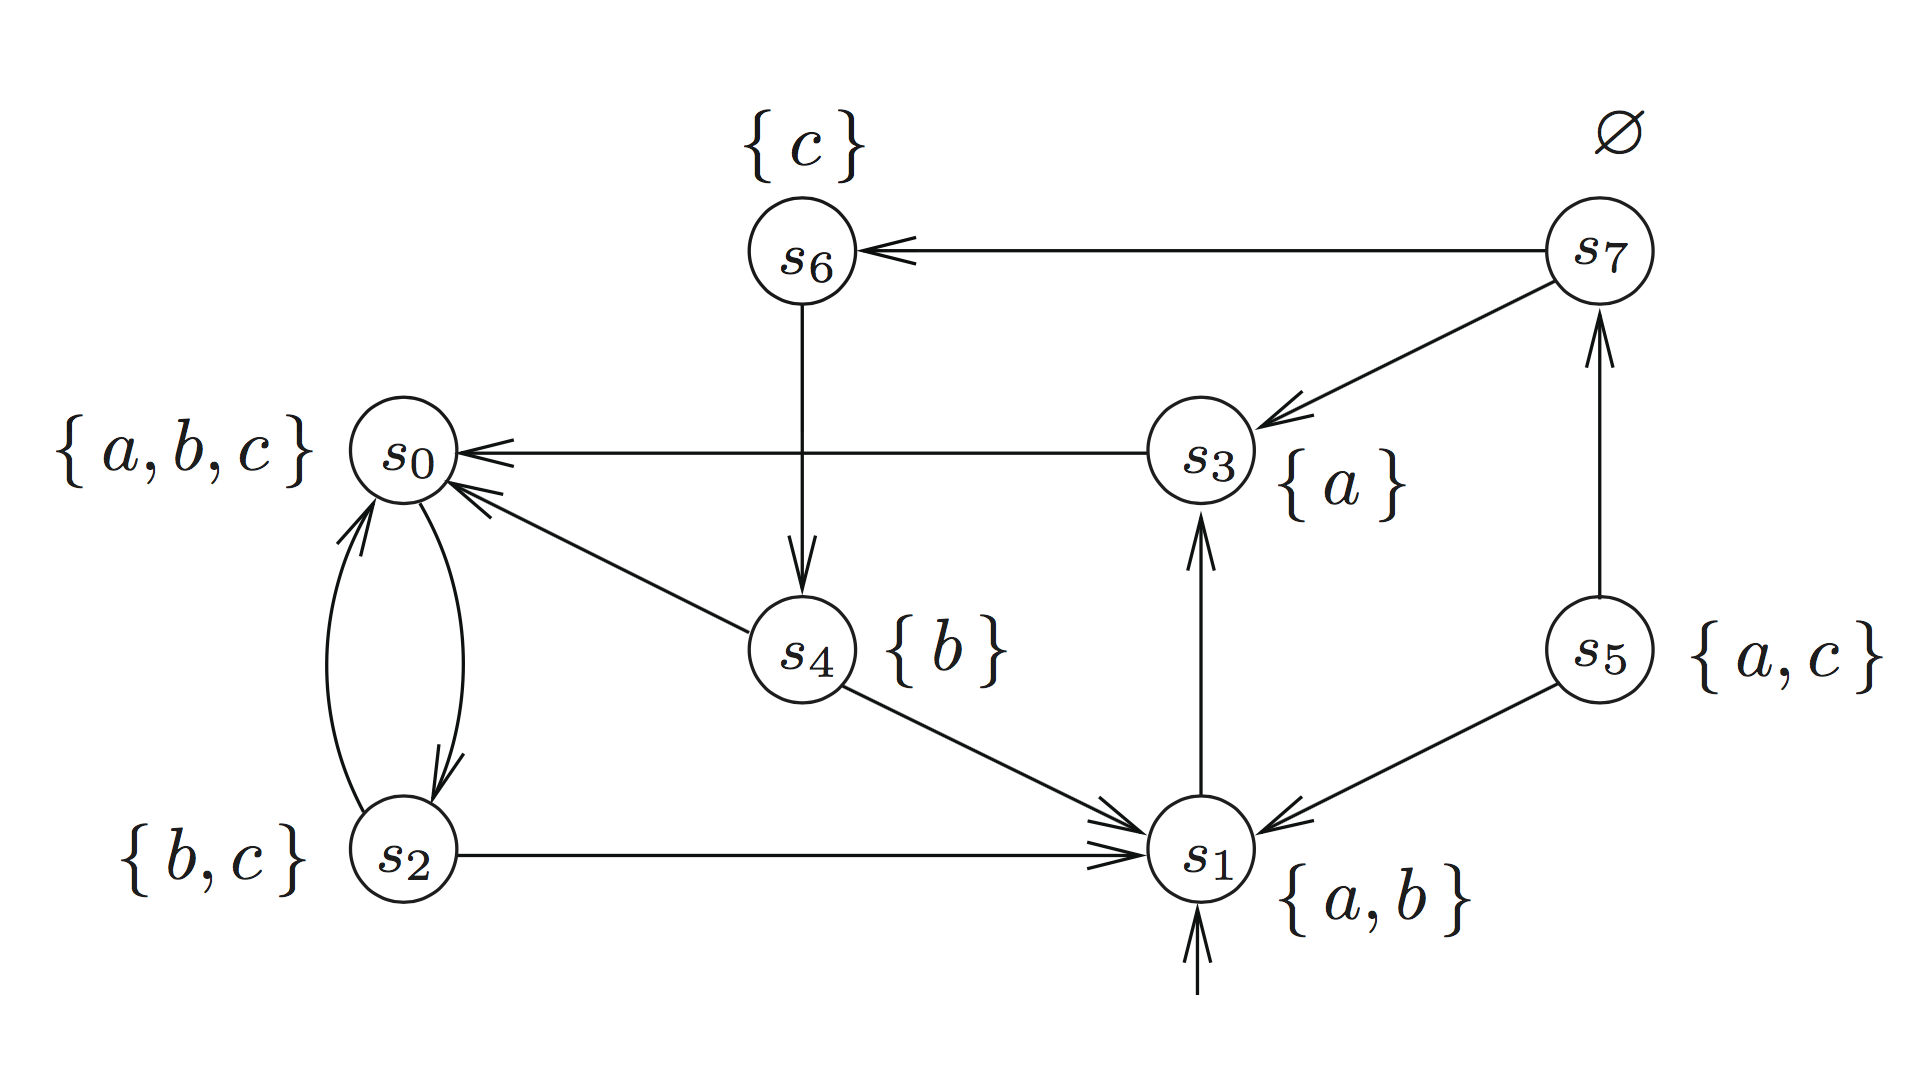
\includegraphics[width=\linewidth]{img/ts.png}
  \caption{Transition system}
  \label{ts6}
\end{figure}
\begin{figure}
  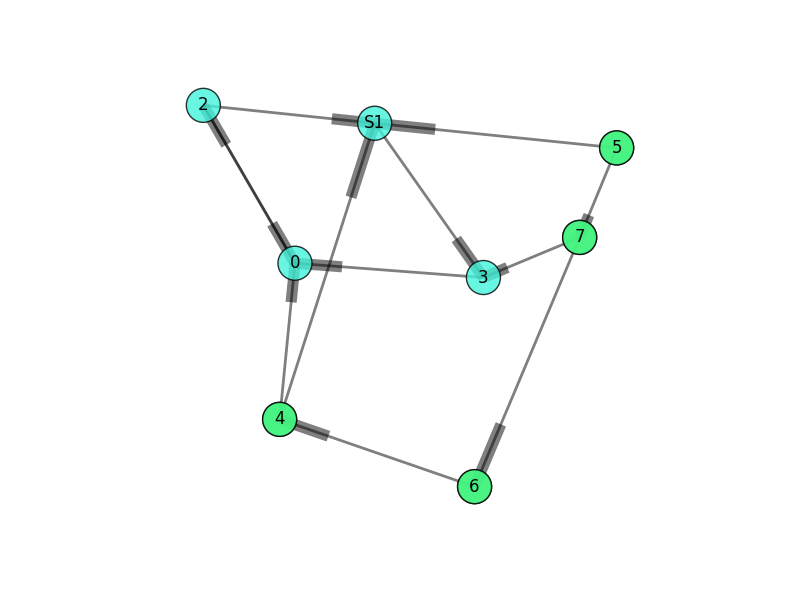
\includegraphics[width=\linewidth]{img/tsResult.png}
  \caption{Transition system risultante}
  \label{tsResult1}
\end{figure}

\subsection{Formula $ \exists \square b$}
La formula in questo caso è già in \ac{ENF} quindi il convertitore non la modifica.
$ \exists \square b$ equivale a

$$[] b$$
e il modelChecker restituisce 
$$(\text{False}, ['0', '2', '4'])$$.
Il risultato in questo esempio si mostra in Figura~\ref{tsResult2}
\begin{figure}
  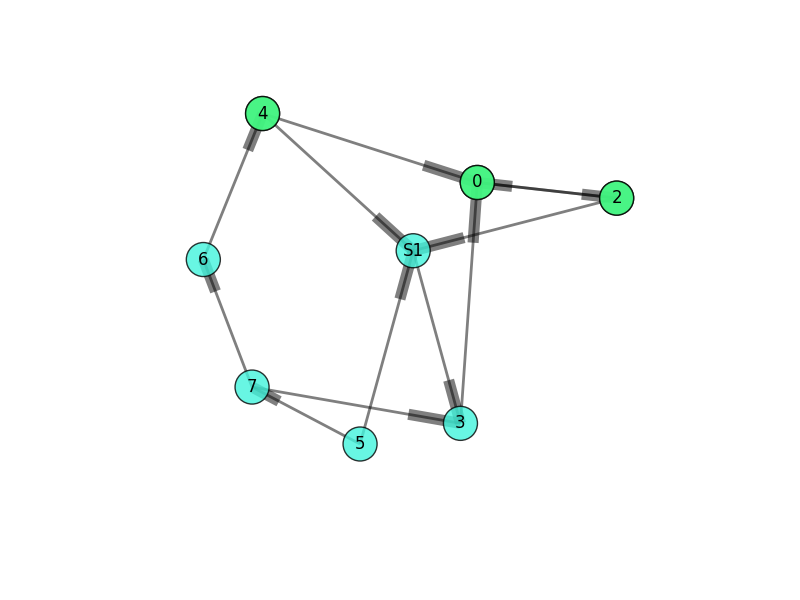
\includegraphics[width=\linewidth]{img/tsResult2.png}
  \caption{Transition system risultante}
  \label{tsResult2}
\end{figure}

\subsection{Fisolofi a cena}

Lo script creato per modellare il problema dei fisolofi a cena, dato in input un intero $n$ restituisce il \ac{GEXF} che rappresenta il \ac{TS} con $n$ filosofi.
Le proposizioni atomiche del \ac{TS} generato sono:
$$AP = \{e_0, \dots, e_n, t_0, \dots, t_n, h_0, \dots, h_n, w_0, \dots, w_n \}$$
che rappresentano gli stati possibili in cui si può trovare ognuno degli $n$ filosofi:
\begin{itemize}
  \item{$t_0 \dots t_n$ rappresentano le proposizioni atomiche dove il filosofo è nello stato "thinking", cioè quando non è in attesa di niente}
  \item{$h_0 \dots h_n$ rappresentano le proposizioni atomiche dove il filosofo è nello stato "hungry", ovvero quando richiede la prima forchetta}
  \item{$w_0 \dots w_n$ rappresentano le proposizioni atomiche dove il filosofo è nello stato "wait", ovvero quando è in attesa della seconda forchetta}
  \item{$e_0 \dots e_n$ rappresenta le prooposizioni atomiche dove il filosofo è nello stato "eating", ovvero quando mangia}
\end{itemize}
Lo stato iniziale del \ac{TS} generato sarà lo stato che conterrà come label l'insieme $\{t_0 \dots t_n\}$, cioè quando tutti i filosofi sono nello stato di "thinking".







%sistemare gli acronimi in una sezione
\section*{Lista di acronimi}
\begin{acronym}
\acro{CTL}{Computational Tree Logic}
\acro{LTL}{Linear Temporal Logic}
\acro{TS}{Transition System}
\acro{ENF}{Existential Normal Form}
\acro{XML}{eXtensible Markup Language}
\acro{GEXF}{Graph Exchange \ac{XML} Format}
\end{acronym}

\end{document}
